\chapter{VLAN and STP}

\section{VLAN}
By default, a device connected to a switch has level-2 connectivity to all the other devices connected to that switch.
Similarly, in a switched network, all the connected devices have layer-2 connectivity to other connected devices.

For example, Fig.~\ref{fig:No_vlan} shows a switched network that is a single layer-2 domain.

\begin{figure}
\centering
\ifpdf
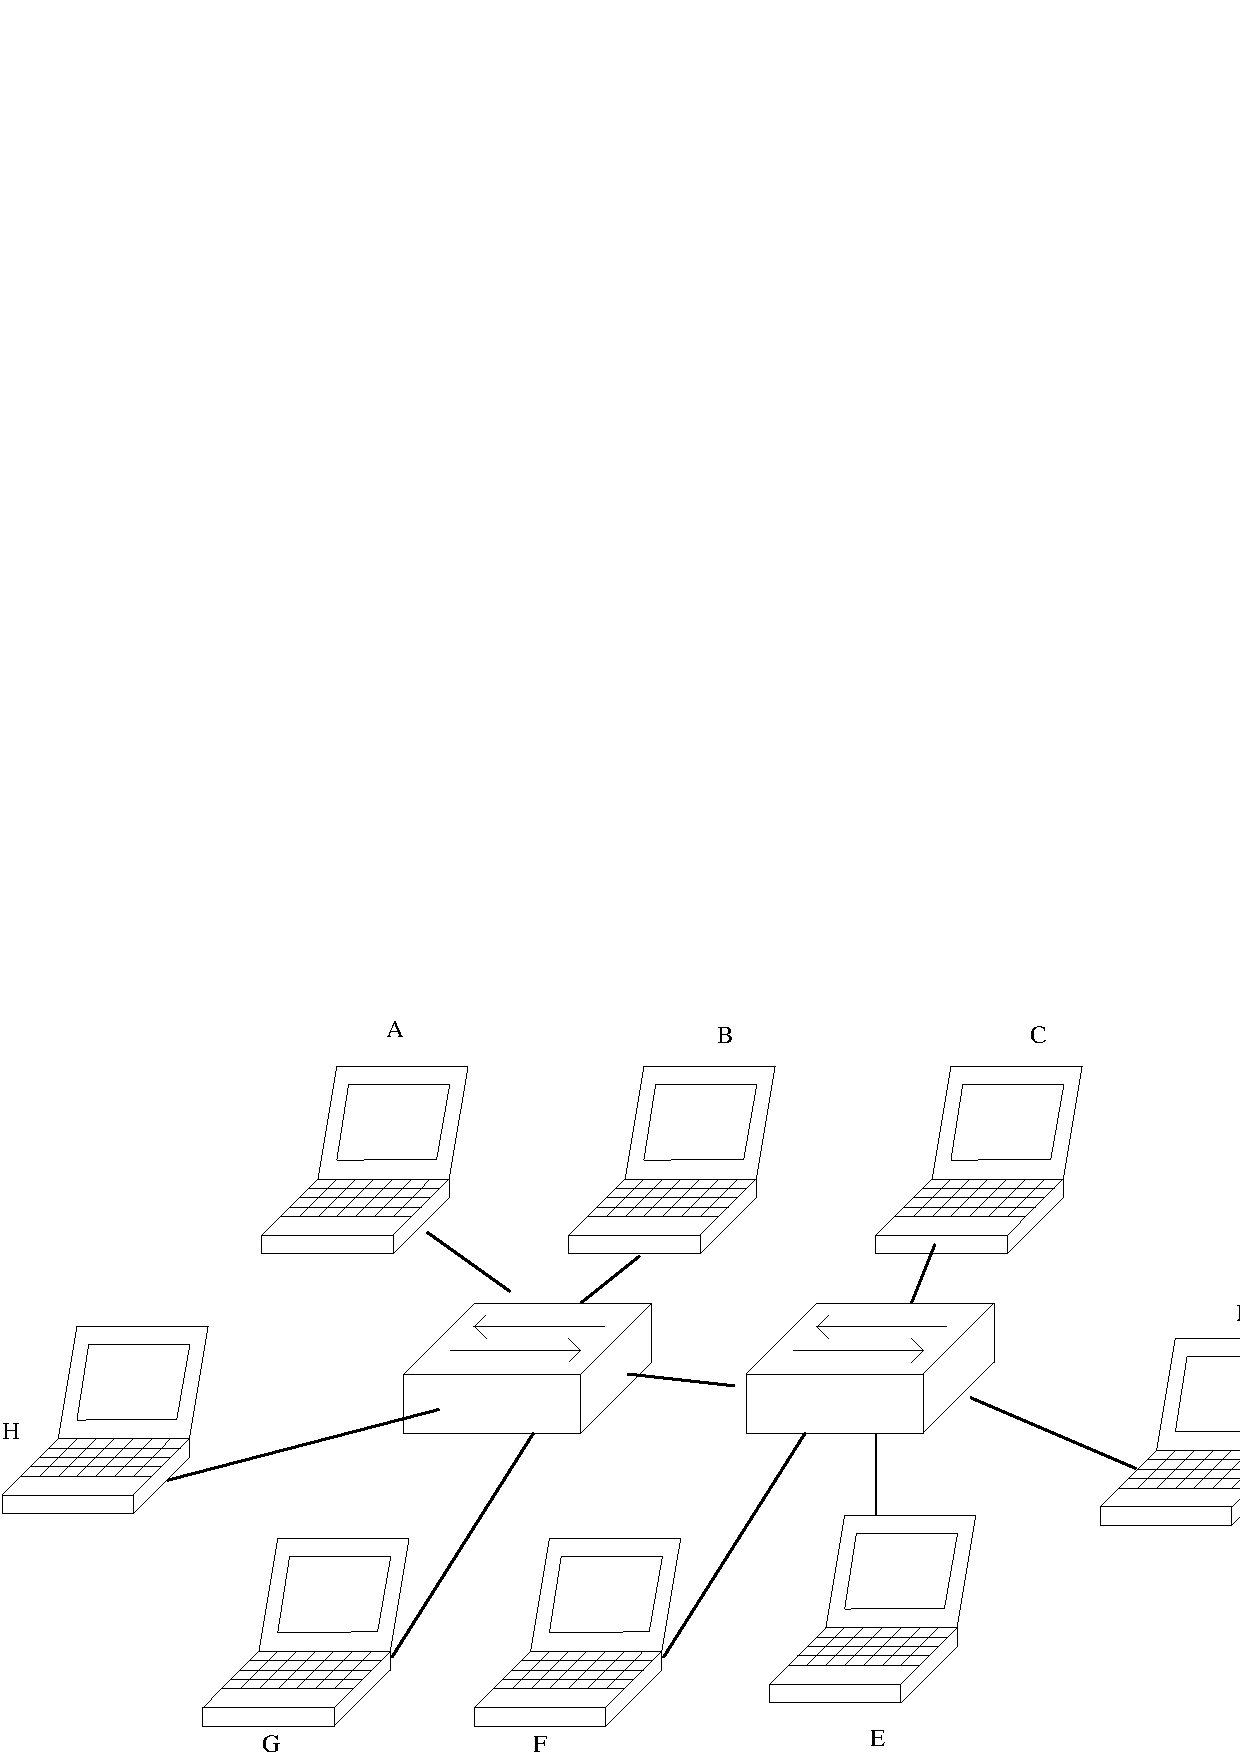
\includegraphics[width=0.5\linewidth]{Figures/No_vlan.pdf}
\else
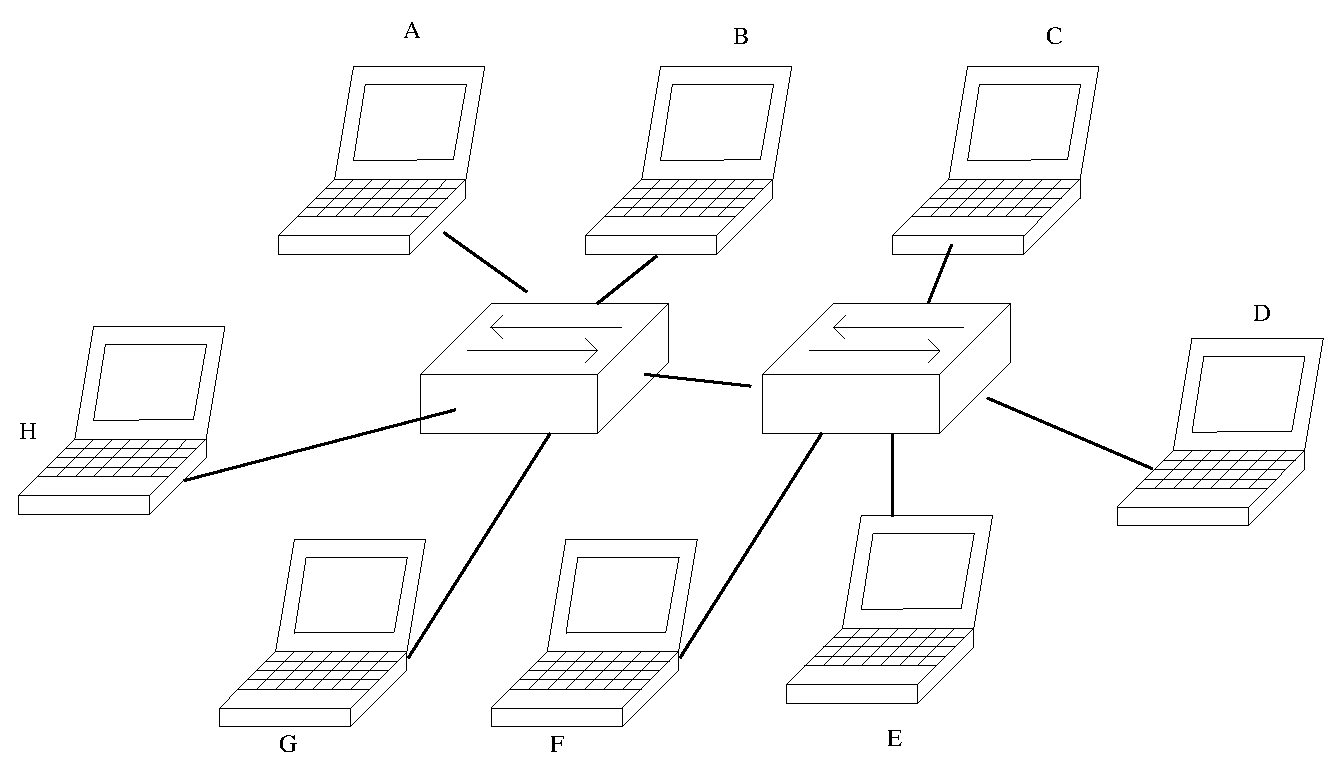
\includegraphics[width=0.5\linewidth]{Figures/No_vlan.eps}
\fi
\caption{A switched network with no VLANs.}
\label{fig:No_vlan}
\end{figure}

There are situations in which it is required to partition the network.
For example, in a campus university it might be necessary to keep wireless access points in a network separated from the servers.
If the access points are separated across multiple buildings, it would be necessary to have a switch for the access points in each building.
Similarly, if there are servers in multiple buildings, it would also be necessary to place a router in each building.
Requiring a switch for every network in every location is a solution that does not scale as the number of locations and networks increase.
It is much more convenient to have a single switch in every location and then configure the switches to keep separate link-layer networks.
This is precisely what VLANs offer.
Fig.~\ref{fig:Vlan} shows an example in which computers A, B and C are kept in a link-layer network separated from D, E and F.


\begin{figure}
\centering
\ifpdf
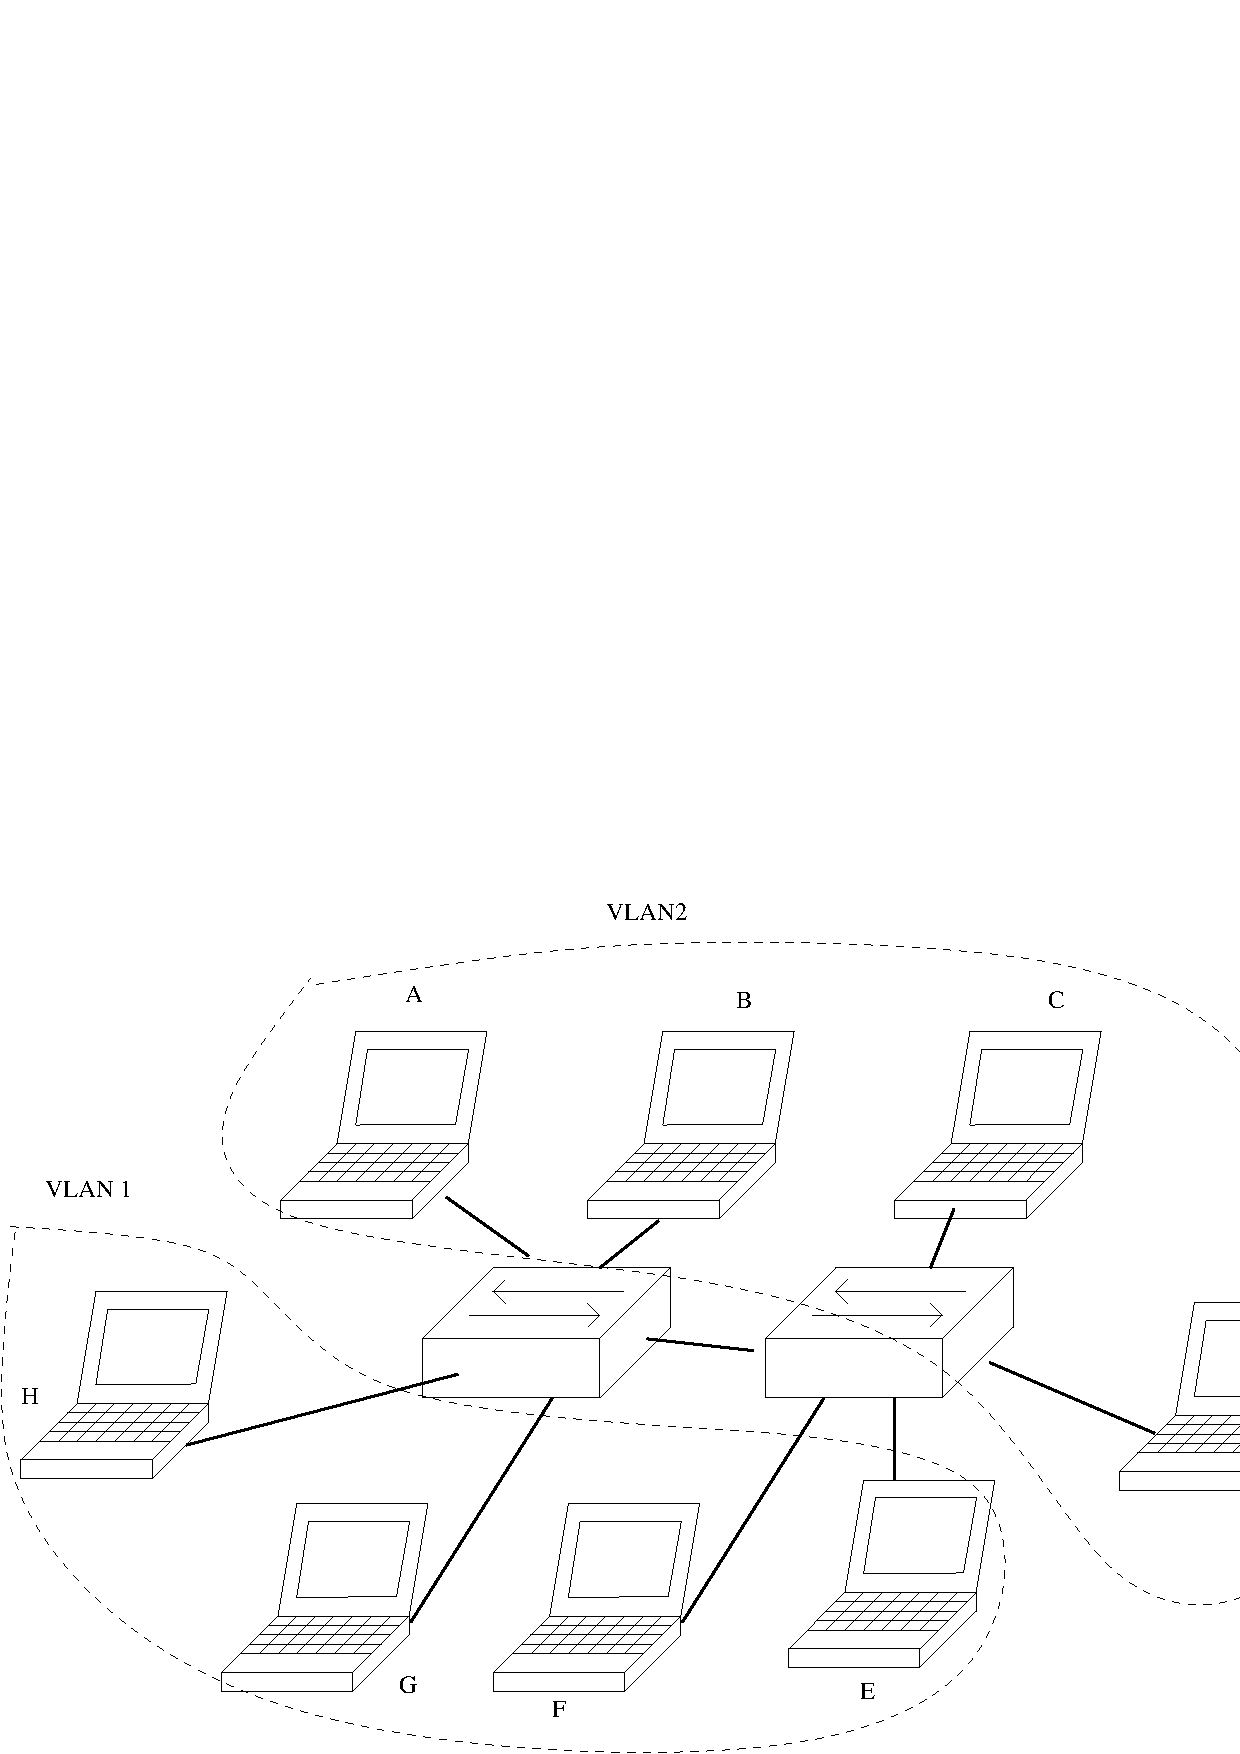
\includegraphics[width=0.5\linewidth]{Figures/Vlan.pdf}
\else
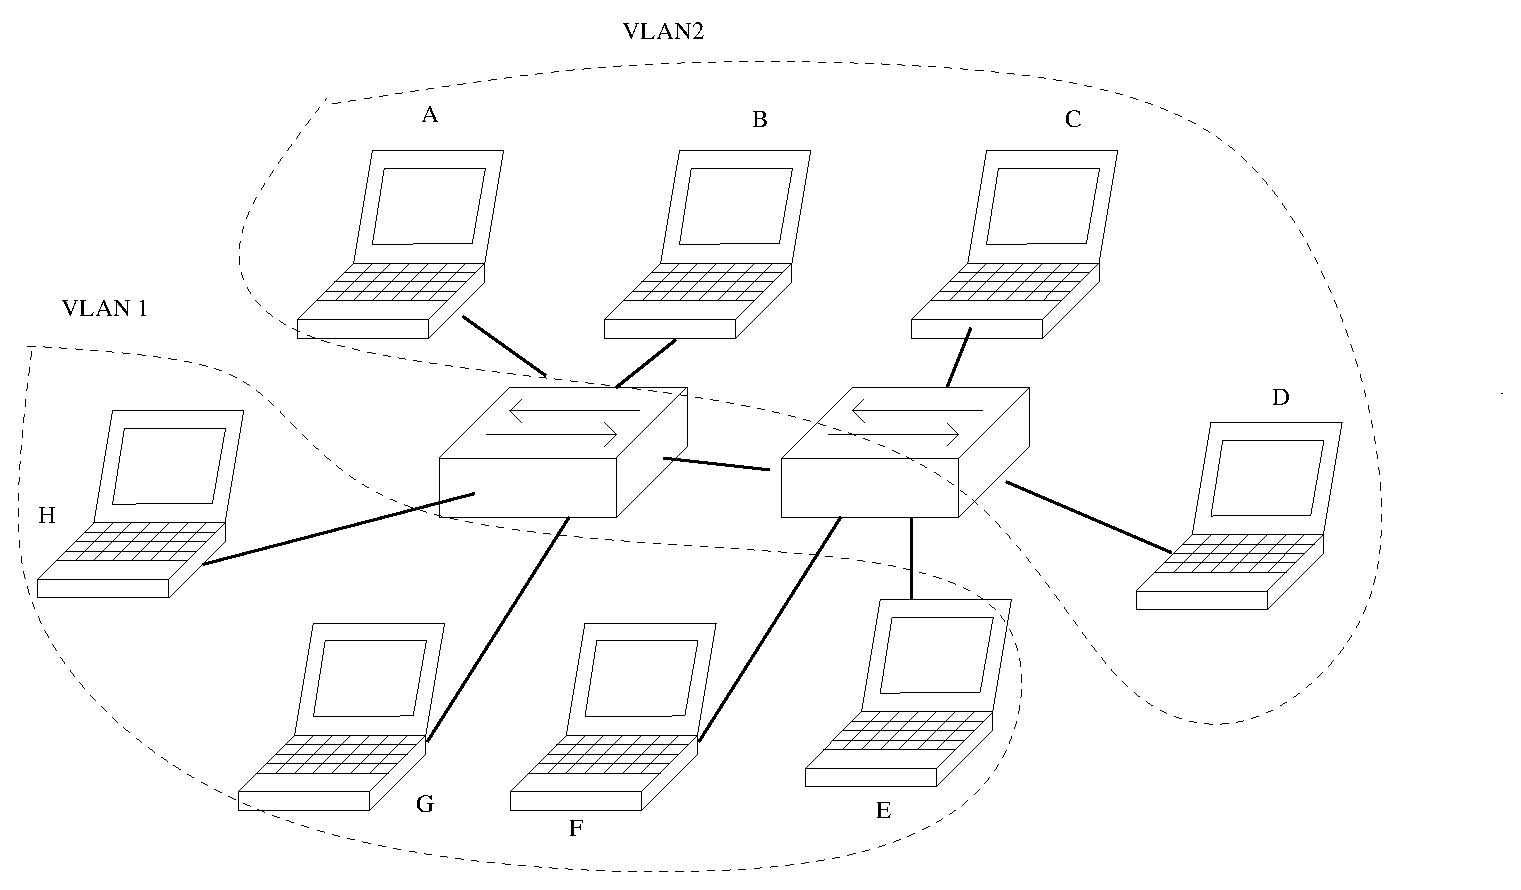
\includegraphics[width=0.5\linewidth]{Figures/Vlan.eps}
\fi
\caption{The network topology used for the STP practical exercise.}
\label{fig:Vlan}
\end{figure}

\begin{figure}
\centering
\ifpdf
\includegraphics[width=0.5\linewidth]{Figures/Equivalent.pdf}
\else
\includegraphics[width=0.5\linewidth]{Figures/Equivalent.eps}
\fi
\caption{The network topology used for the STP practical exercise.}
\label{fig:Equivalent}
\end{figure}


